\chapter{Introducción Específica} % Main chapter title

\label{Chapter2}

%----------------------------------------------------------------------------------------
%	SECTION 1
%----------------------------------------------------------------------------------------

El presente capítulo presenta los requerimientos del dispositivo, una descripción de los bloques que lo componen y la planificación que se siguió para lograr satisfactoriamente el desarrollo.

%----------------------------------------------------------------------------------------

\section{Requerimientos}

El dispositivo tiene dos tipos de requerimientos, funcionales y no funcionales. Los funcionales, se refieren a la capacidad para cumplir con ciertas tareas impuestas, que garantizan un correcto desempeño del dispositivo en general. Los no funcionales, tienen relación con temas de carácter económico e informativo.

\subsection{Requerimientos funcionales}

\begin{itemize}
	\item El dispositivo deberá poseer conexión Wi-Fi\footnote{Wi-Fi. Es una tecnología inalámbrica para la interconexión de dispositivos electrónicos.}
	\item El dispositivo deberá funcionar como servidor web local.
	\item El dispositivo deberá contar con la hora y fecha exactas.
	\item El dispositivo deberá interpretar los pulsos ópticos provenientes de un medidor de consumo de energía eléctrica domiciliario.
	\item El dispositivo deberá poseer una memoria no volátil para registrar datos como la hora, fecha, conteo de pulsos e ID del usuario; durante al menos tres meses.
	\item El dispositivo deberá contar con un sistema de adquisición, procesamiento, transmisión y recepción de datos, el mismo podrá ser implementado en un microcontrolador con Wi-Fi integrado.
	\item El dispositivo deberá poseer una interfaz web para que los usuarios puedan observar un registro histórico de su consumo de energía eléctrica.
	\item El dispositivo deberá poder establecer conexión con un gateway LoRa, para enviar diariamente en formato hexadecimal la hora, fecha, consumo de energía eléctrica e ID del usuario.
\end{itemize}

\subsection{Requerimientos no funcionales}

\begin{itemize}
	\item El dispositivo deberá tener un precio menor a 50 \$us.
	\item El dispositivo deberá contar con manuales de uso e instalación.
\end{itemize}

%----------------------------------------------------------------------------------------

\section{Esquema general del sistema}

Para cumplir con todos los requerimientos funcionales expuestos en la sección anterior, los componentes mínimos necesarios y su interconexión se muestran en el diagrama en bloques de la figura 2.1.

\begin{figure}[h]
	\centering
	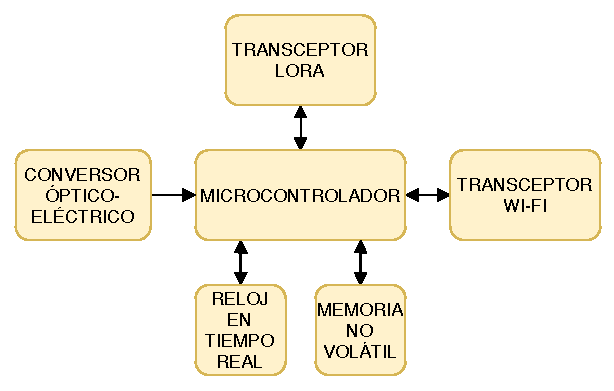
\includegraphics[scale=1]{./Figures/general_blocks.pdf}
	\caption{Diagrama en bloques general del dispositivo.}
	\label{fig:cuadradoAzul}
\end{figure}

En el diagrama anterior, el conversor óptico-eléctrico, transforma los pulsos de luz provenientes del LED de un  medidor de consumo eléctrico a pulsos eléctricos y los entrega al microcontrolador. El microcontrolador procesa estos pulsos y realiza el cálculo del consumo eléctrico, esa información junto con la hora y fecha provenientes del reloj en tiempo real, son almacenados en la memoria no volátil para su posterior utilización. El transceptor Wi-Fi, se comunica con el microcontrolador para obtener los datos que serán utilizados para generar la interfaz gráfica mostrada al usuario. El transceptor LoRa, tiene la función de establecer comunicación bidireccional con un dispositivo concentrador LoRa, para enviar la información de la memoria no volátil y recibir parámetros de funcionamiento.

\subsection{Conversor óptico-eléctrico}

Es el encargado de convertir la salida de pulso óptico de medidores eléctricos digitales a pulsos eléctricos, para que puedan ser interpretados por un microcontrolador. Esta información determina el consumo eléctrico que registra el medidor.

La salida de pulso óptico de los medidores eléctricos digitales, esta compuesta por un LED de color rojo, que emite luz cuando se ha consumido una cierta cantidad de kWh. El valor de la relación entre los pulsos emitidos y el consumo eléctrico, es un parámetro intrínseco del medidor, que varía según el modelo y la firma que lo fabrica.

Para realizar la conversión de pulsos de luz a pulsos eléctricos, existen principalmente dos transductores que cumplen cabalmente esta función:

\begin{itemize}
	\item Fotoresistencia: es una resistencia cuyo valor se modifica en función a la intensidad de luz incidente. También es conocida como LDR (\textit{Light-Dependent Resistor}, resistencia dependiente de la luz) \citep{BOOK:2}. En la figura 2.2 se observa una fotoresistencia.
	
	\begin{figure}[h]
		\centering
		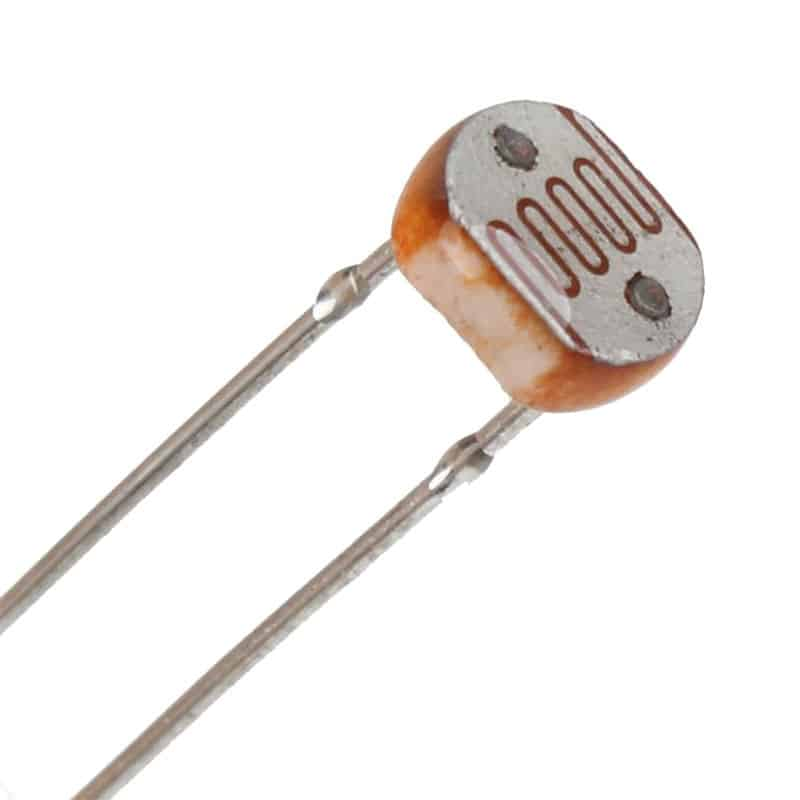
\includegraphics[scale=0.15]{./Figures/ldr.jpg}
		\caption{Fotoresistencia GL5528\protect\footnotemark.}
		\label{fig:cuadradoAzul}
	\end{figure}
	
	\footnotetext{Imagen tomada de: \url{https://www.devobox.com/en/photosensors/38-photoresistor-ldr07.html}}
	
	\item Fototransistor: es un transistor sensible a la luz, normalmente a los infrarrojos. La cantidad de luz incidente es proporcional a la corriente de base generada. Generalmente tiene el factor de forma de un LED \citep{BOOK:2}. Un fototransistor de uso común se observa en la figura 2.3.
\end{itemize}

	\begin{figure}[h]
		\centering
		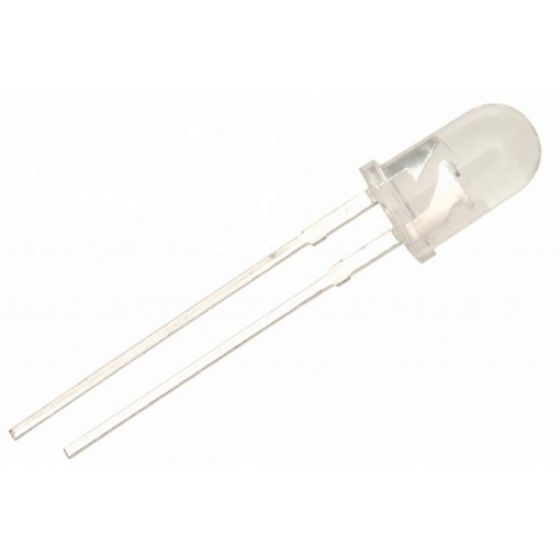
\includegraphics[scale=0.3]{./Figures/phototransistor.jpg}
		\caption{Fototransistor IR333C\protect\footnotemark.}
		\label{fig:cuadradoAzul}
	\end{figure}

	\footnotetext{Imagen tomada de: \url{https://www.steren.com.gt/fototransistor-de-5-mm-transparente.html}}

\subsection{Microcontrolador}

Un microcontrolador es un circuito integrado programable, capaz de ejecutar las instrucciones que tiene almacenadas. Dispone de los tres componentes básicos de de una computadora: memoria, CPU(\textit{Central Processing Unit}, unidad central de procesamiento) y periféricos de entrada/salida. 

El diseño de los microcontroladores está orientado a reducir los cotos económicos y el consumo energético de un sistema en particular. Según la aplicación en la que el microcontrolador se vaya a utilizar, el tamaño de la unidad central de procesamiento, la cantidad de memoria y los periféricos incluidos son diferentes. Es por esta razón que tiene recursos de hardware muy limitados en comparación con, por ejemplo, una computadora.

Los fabricantes más populares de microcontroladores son: Analog Devices, Cypress Semiconductor, Infineon, Maxim Integrated, Microchip, NXP, On Semiconductor, Panasonic, ROHM Semiconductor, STMicroelectronics y Texas Instruments \citep{WEBSITE:12}.

En el mercado se pueden encontrar microcontroladores en diferentes factores de forma, pero, para el desarrollo de sistemas embebidos, lo más común es utilizar tarjetas de desarrollo como la que se muestra en la figura 2.x.

\begin{figure}[h]
	\centering
	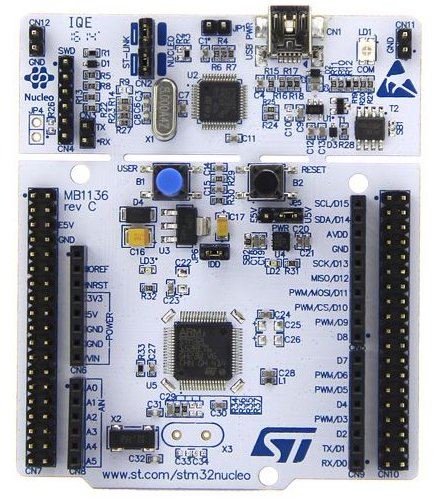
\includegraphics[scale=0.4]{./Figures/microcontroller_dev.jpg}
	\caption{Tarjeta de desarrollo del fabricante STMicroelectronics basada en el microcontrolador STM32F030R8T6\protect\footnotemark.}
	\label{fig:cuadradoAzul}
\end{figure}

\footnotetext{Imagen tomada de: \url{https://www.seeedstudio.com/NUCLEO-L152RE-Development-Board-for-STM32-p-1934.html}}

\subsection{Transceptor Wi-Fi}

Wi-Fi es un tecnología de red inalámbrica, que permite a dispositivos como computadoras y teléfonos celulares conectarse entre sí para formar una red, o conectarse a un enrutador por el que se disponga de conexión a Internet. Está basado en la familia de estándares IEEE 802.11, que definen los protocolos que permiten la comunicación entre dispositivos compatibles con Wi-Fi \citep{WEBSITE:11}.Según la versión de Wi-Fi, puede funcionar en las bandas de 2.4 GHz o 5 GHz\citep{WEBSITE:11}.

En la tabla 2.1 muestran las características técnicas de las distintas versiones del estándar IEEE 802.11.

\begin{table}[h]
	\centering
	\caption[IEEE 802.11]{Tabla comparativa de características del estándar IEEE 802.11\protect\footnotemark}
	\begin{tabular}{l c c c}    
		\toprule
		\textbf{Protocolo 802.11} & \textbf{Frecuencia} & \textbf{Ancho de banda} & \textbf{Velocidad de datos (Mb/s)} \\
		\midrule
		a & 5 GHz 			& 20 MHz 		  & 5, 9, 12, 18, 24, 36, 48, 54 \\		
		b & 2.4 GHz			& 20 MHz 		  & 1, 2, 5.5, 11 \\
		g & 2.4 GHz			& 20 MHz          & 6, 9, 12, 18, 24, 36, 48, 54 \\
		n & 2.4 GHz y 5 GHz & 20 MHz y 40 MHz & 7.2, 28.9, 43.3, 57.8, 65, 72.2 \\
		\bottomrule
		\hline
	\end{tabular}
	\label{tab:peces}
\end{table}

\footnotetext{Datos obtenidos de: \url{https://microchipdeveloper.com/wifi:a-b-g-n-explained}}

Dentro del modelo OSI\footnote{Modelo OSI. Es un modelo de referencia para los protocolos de red, creado por la Organización Internacional de Normalización.}, Wi-Fi se encuentra en la capa física y de enlace de datos. En la figura 2.x se ve el modelo OSI.
\begin{figure}[h]
	\centering
	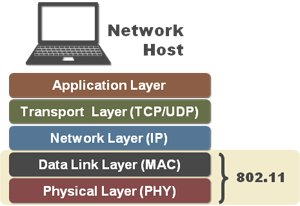
\includegraphics[scale=0.7]{./Figures/osi_model.jpg}
	\caption{Ubicación de Wi-Fi en el modelo OSI\protect\footnotemark.}
	\label{fig:cuadradoAzul}
\end{figure}

\footnotetext{Imagen tomada de: \url{https://microchipdeveloper.com/wifi:80211-osi}}

Una red Wi-Fi tiene una arquitectura en estrella como se muestra en la figura 2.x. 

\begin{figure}[h]
	\centering
	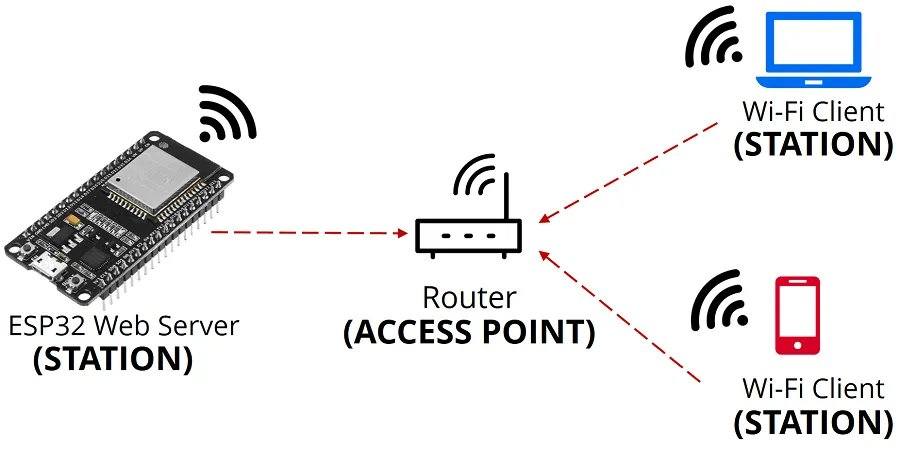
\includegraphics[scale=0.33]{./Figures/wifi_architecture.jpg}
	\caption{Arquitectura de una red Wi-Fi\protect\footnotemark.}
	\label{fig:cuadradoAzul}
\end{figure}

\footnotetext{Imagen tomada de: \url{https://randomnerdtutorials.com/esp32-access-point-ap-web-server/}}

Los elementos principales de una red Wi-Fi son:
\begin{itemize}
	\item Estaciones: son dispositivos electrónicos que se conectan entre sí a través de enrutadores inalámbricos. Son más conocidos como \textit{hosts} y pueden ser computadoras, tabletas, teléfonos celulares o sistemas embebidos.
	\item Puntos de acceso: también conocidos como \textit{access points}, son los elementos de la red que enrutan la información proveniente de las estaciones dentro de la red local o hacia otras redes.
\end{itemize}

Dentro de lo referido al desarrollo de sistemas embebidos, comercialmente pueden encontrarse módulos Wi-Fi como el de la figura 2.x.

\begin{figure}[h]
	\centering
	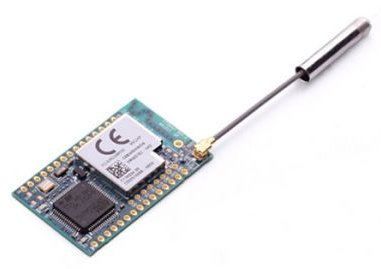
\includegraphics[scale=0.3]{./Figures/wifi_module.jpg}
	\caption{Módulo Wi-Fi basado en el circuito integrado EMW3162\protect\footnotemark.}
	\label{fig:cuadradoAzul}
\end{figure}

\footnotetext{Imagen tomada de: \url{https://www.seeedstudio.com/EMW3162-WiFi-Module-External-IPEX-antenn-p-2235.html}}

\subsection{Transceptor LoRa}

LoRa(\textit{Long Range}, largo alcance), es una técnica de modulación de espectro extendido derivada de la tecnología CSS (\textit{Chirp Spread Spectrum}, espectro extendido de tipo chirp)\citep{WEBSITE:9}. Fue desarrollado por la firma Semtech y es utilizada principalmente en dispositivos orientados a IoT(\textit{Internet of Things}, Internet de las cosas) y dispositivos alimentados por baterías. Opera en las bandas de 433 Mhz, 868 Mhz y 915 MHz, según el país.

Las comunicaciones entre dispositivos LoRa, son del tipo punto a punto, ya que la tecnología es de capa física. Para formar redes LoRa, es necesaria una capa MAC (\textit{Media Access Control}, control de acceso al medio), la cual es llamada LoRaWAN (\textit{Long Range Wide Area Network}, red de área amplia LoRa).

LoRaWAN, es una especificación de redes LPWAN (\textit{Low Power Wide Area Network}, red de área amplia de baja potencia) y LoRa Alliance es la encargada de su estandarización. Está diseñada para conectar dispositivos de bajo consumo energético a Internet a través de redes regionales, nacionales o globales. Además proporciona comunicación bidireccional, seguridad, movilidad y servicios de localización\citep{WEBSITE:10}.

En la figura 2.x se puede observar el modelo de capas de una red de dispositivos LoRa, donde el protocolo LoRa define la capa física (PHY) y LoRaWAN la capa de acceso al medio (MAC).

\begin{figure}[h]
	\centering
	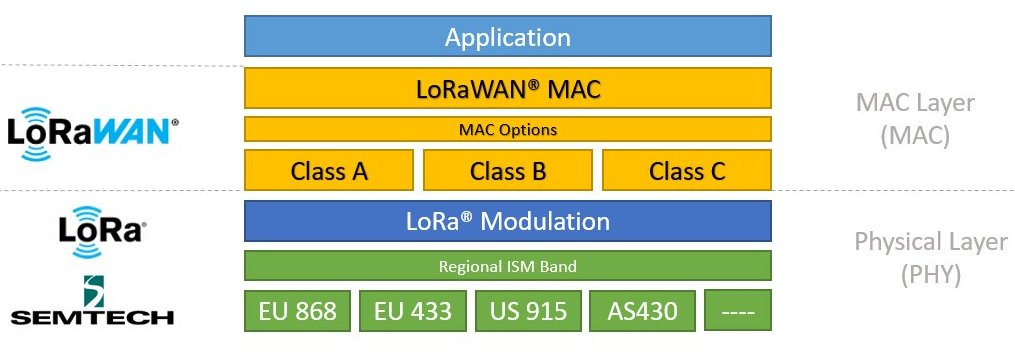
\includegraphics[scale=0.38]{./Figures/lorawan.jpg}
	\caption{\textit{Stack} LoraWAN\protect\footnotemark.}
	\label{fig:cuadradoAzul}
\end{figure}

\footnotetext{Imagen tomada de: \url{https://lora-developers.semtech.com/library/tech-papers-and-guides/lora-and-lorawan/}}

La arquitectura de una red LoRaWAN es de tipo estrella, como se muestra en la figura 2.x.

\begin{figure}[h]
	\centering
	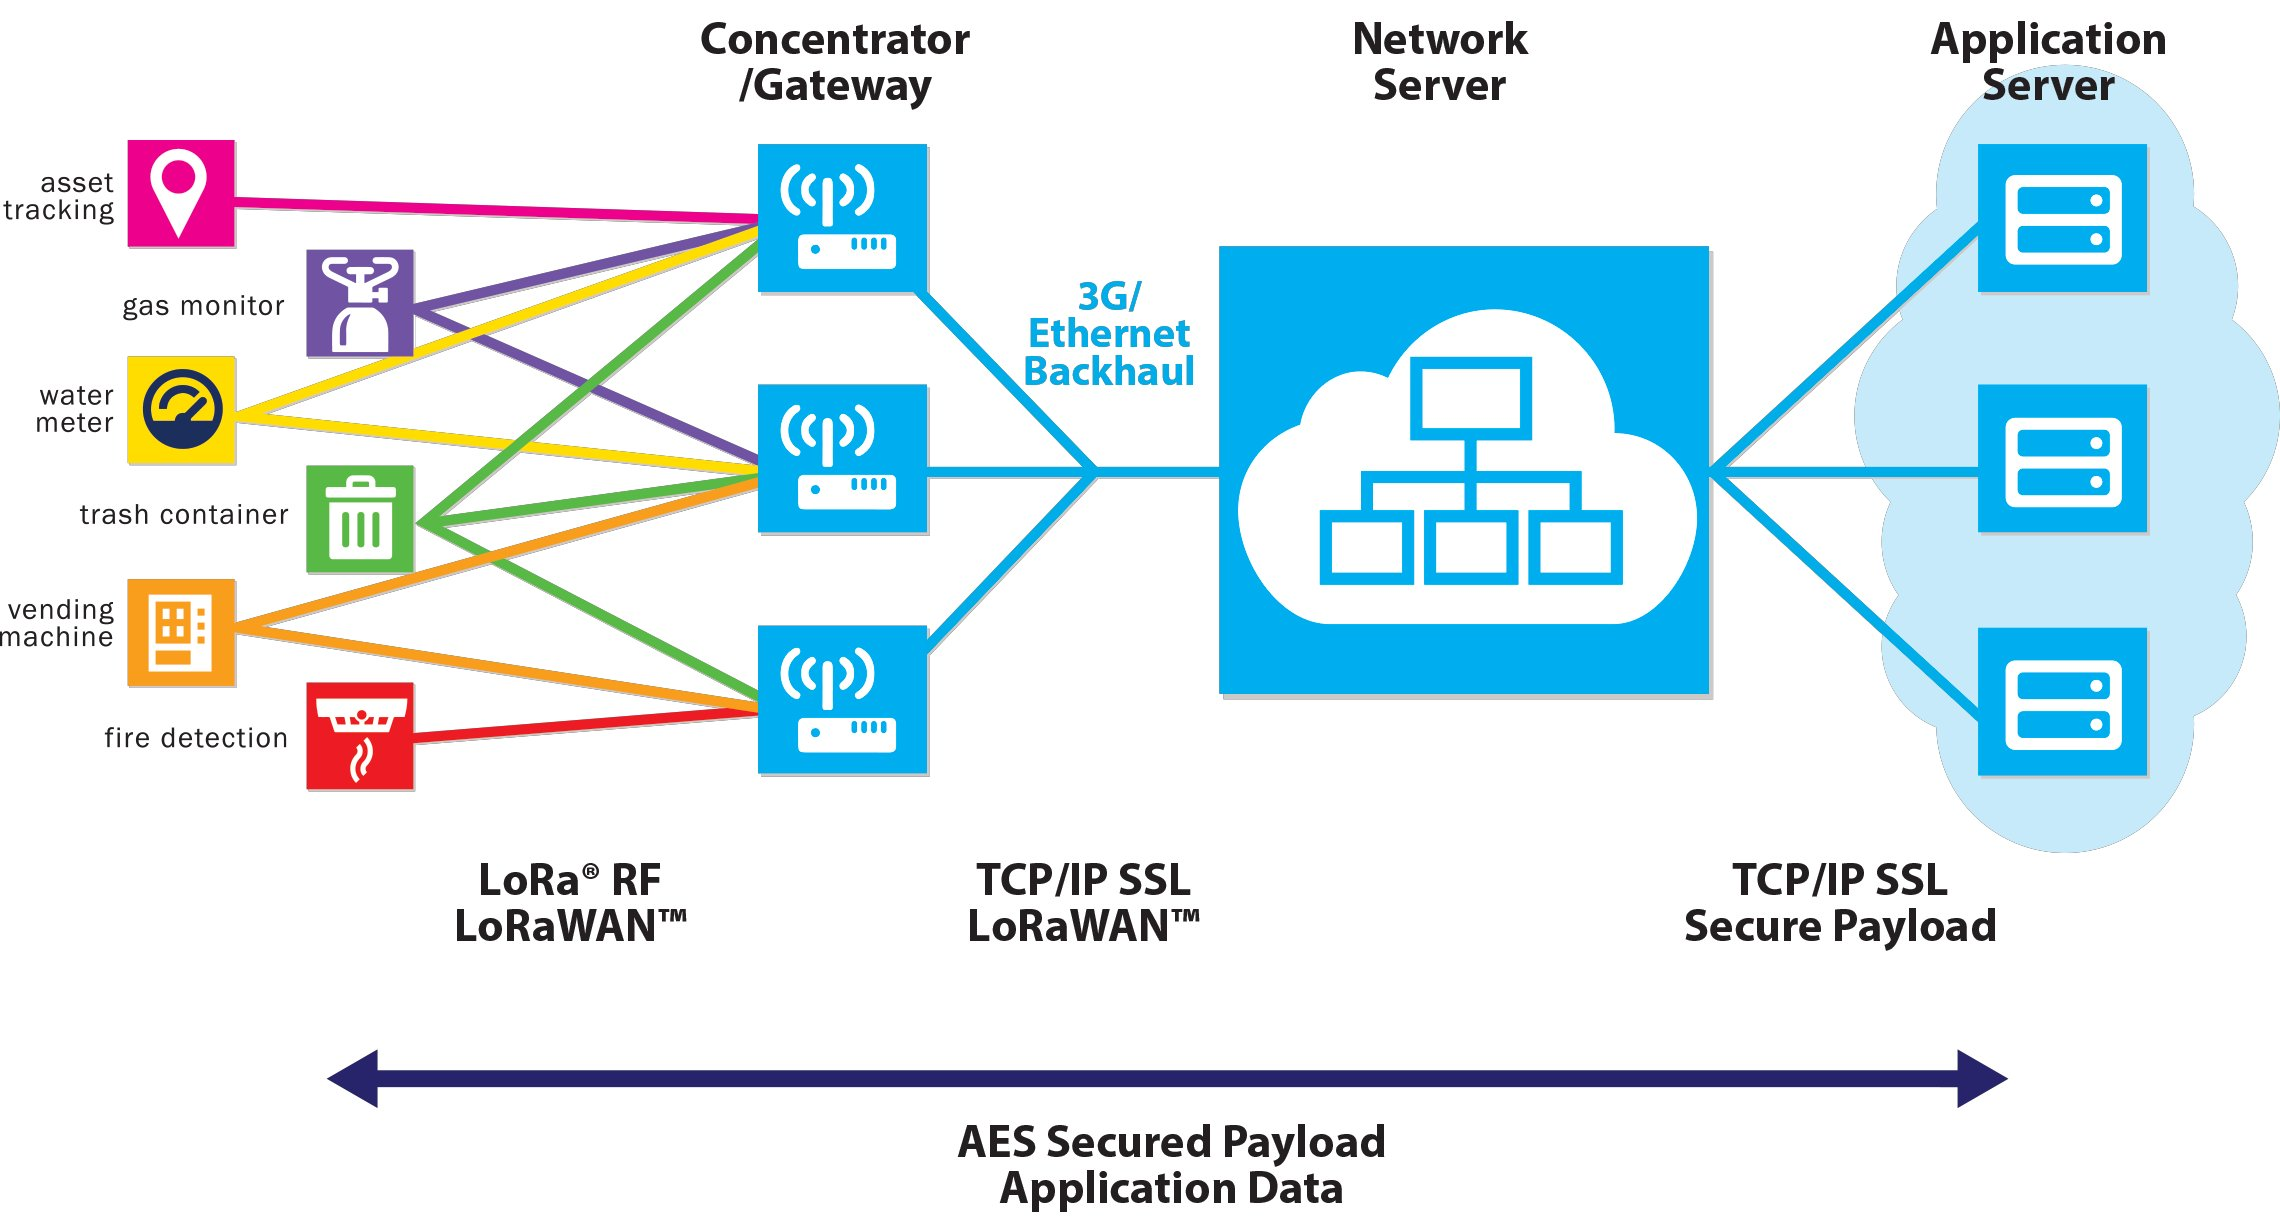
\includegraphics[scale=0.17]{./Figures/lorawan_architecture.jpg}
	\caption{Arquitectura de una red LoraWAN\protect\footnotemark.}
	\label{fig:cuadradoAzul}
\end{figure}

\footnotetext{Imagen tomada de: \url{https://www.aprendiendoarduino.com/2018/03/05/redes-lpwan/}}

De la figura anterior, se distinguen los siguientes elementos:

\begin{itemize}
	\item Nodos: son los dispositivos que utilizan la tecnología LoRa como método de transmisión de datos. Son utilizados para obtener datos de sensores o para interactuar con actuadores. Generalmente son dispositivos de bajo consumo energético y alimentados por baterías.
	\item Concentradores: también conocidos como \textit{gateways}, son los encargados de recibir la información de los nodos y reenviarla a un servidor de red. Estos dispositivos tienen acceso a Internet mediante redes celulares, Wi-Fi o \textit{ethernet}.
	\item Servidores de red: son los responsables del enrutamiento de los mensajes a la aplicación adecuada, seleccionar el mejor gateway para el mensaje de enlace descendente, eliminar mensajes duplicados y descifrar los mensajes que vienen cifrados desde los nodos.
	\item Servidores de aplicación: es donde se realizan los procesos útiles sobre los datos obtenidos de los nodos. Típicamente se ejecutan en una nube privada o pública.
\end{itemize}

En el desarrollo de nodos para redes LoRaWAN, se utilizan módulos que llevan embebido un circuito integrado con tecnología LoRa, como el de la figura 2.x.

\begin{figure}[h]
	\centering
	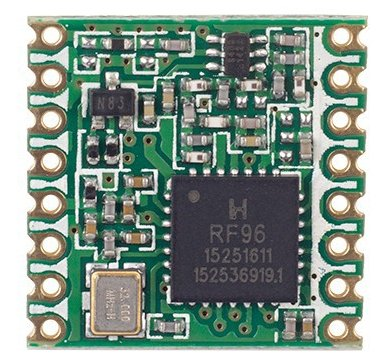
\includegraphics[scale=0.32]{./Figures/lora_module.jpg}
	\caption{Módulo LoRa basado en el circuito integrado RF96\protect\footnotemark.}
	\label{fig:cuadradoAzul}
\end{figure}

\footnotetext{Imagen tomada de: \url{https://www.antratek.com/rfm95-lora-module}}

\subsection{Reloj en tiempo real}

Más conocido como RTC (\textit{Real-Time Clock}, reloj en tiempo real), es un circuito integrado que tiene la capacidad de llevar con precisión la hora y fecha. Para contar con exactitud los segundos, utiliza un oscilador de cristal de cuarzo de 32.768 kHz, que puede o no estar embebido en el encapsulado del RTC.

La principal aplicación de un RTC es brindar a un sistema electrónico la hora y fecha exactas,  también puede ofrecer otras funciones como alarmas, salidas de reloj de 1 Hz o medición de temperatura.

Algunos RTCs tienen una fuente de poder alternativa basada en baterías, que mantiene funcionando la parte del circuito que lleva la cuenta de la hora y fecha. Esta fuente de tensión normalmente son baterías de litio o supercapacitores\footnote{Supercapacitor. Es un capacitor que tiene valores de capacitancia muy altos, pero valores de voltaje muy bajos.}. Comercialmente un RTC puede adquirirse como parte de un módulo, como el que se ve en la figura 2.4, que tiene instalada la fuente de alimentación alternativa y brinda mayor facilidad para acceder a los pines del circuito integrado.

\begin{figure}[h]
	\centering
	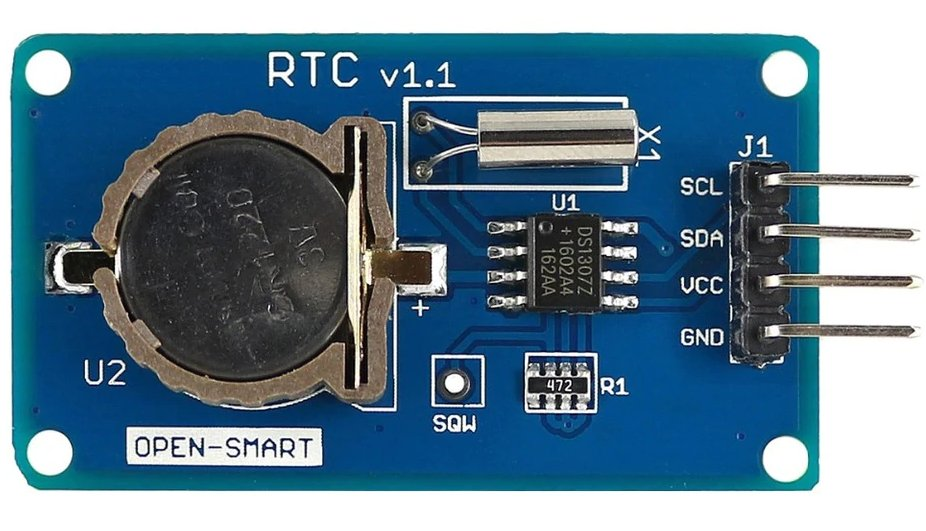
\includegraphics[scale=0.2]{./Figures/rtc.jpg}
	\caption{Módulo RTC basado en el circuito integrado DS1307\protect\footnotemark.}
	\label{fig:cuadradoAzul}
\end{figure}

\footnotetext{Imagen tomada de: \url{https://www.antratek.com/rfm95-lora-module}}

\subsection{Memoria no volátil}

Es un tipo de memoria de lectura y escritura, en la que los datos que tiene almacenados se mantienen intactos cuando la fuente de alimentación deja de funcionar, es decir, que no necesita energía para mantener guardada la información grabada en ella \citep{BOOK:3}.

En sistemas embebidos, existen principalmente dos tipos de memorias no volátiles:

\begin{itemize}
	\item EEPROM (\textit{Electrically Erasable Programmable Read-Only Memory}, ROM borrable y programable eléctricamente): es un tipo de memoria ROM que puede ser programada y borrada mediante métodos eléctricos. Aunque puede ser leída un número ilimitado de veces, las operaciones de escritura o borrado de datos solo se pueden realizar entre cien mil y un millón de veces. Este tipo de memorias pueden encontrarse como circuitos integrados que generalmente disponen de comunicación I2C o SPI. En la figura 2.5 se aprecia un módulo EEPROM, comercialmente esta es la forma más habitual de encontrarlo.
	\begin{figure}[h]
		\centering
		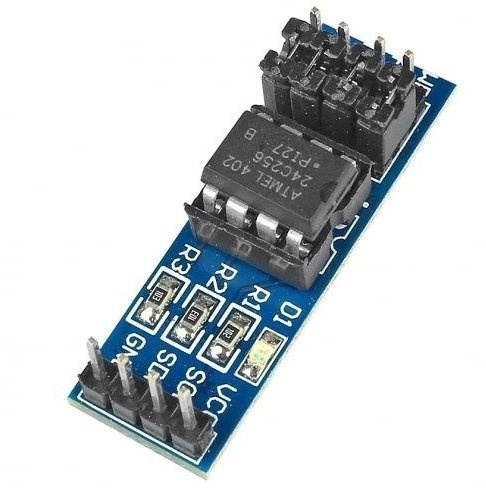
\includegraphics[scale=0.35]{./Figures/eeprom.jpg}
		\caption{Módulo EEPROM basado en el circuito integrado 24C256\protect\footnotemark.}
		\label{fig:cuadradoAzul}
	\end{figure}

	\footnotetext{Imagen tomada de: \url{https://www.antratek.com/rfm95-lora-module}}

	\item Flash: está basada en las memorias EEPROM y permite la lectura y escritura de múltiples posiciones de memoria de manera simultánea, gracias a ello su velocidad de funcionamiento es superior a la de su antecesor. El número de operaciones de escritura o borrado es de diez mil a un millón. Es empleada principalmente en la fabricación de memorias USB y unidades de estado sólido. Asimismo, los microcontroladores actuales tienen integrada una unidad de memoria flash para el almacenamiento de instrucciones y datos. Para la realización de pruebas y prototipos, existen comercialmente módulos de memoria flash con comunicación SPI, como el de la figura 3.6.
	\begin{figure}[h]
		\centering
		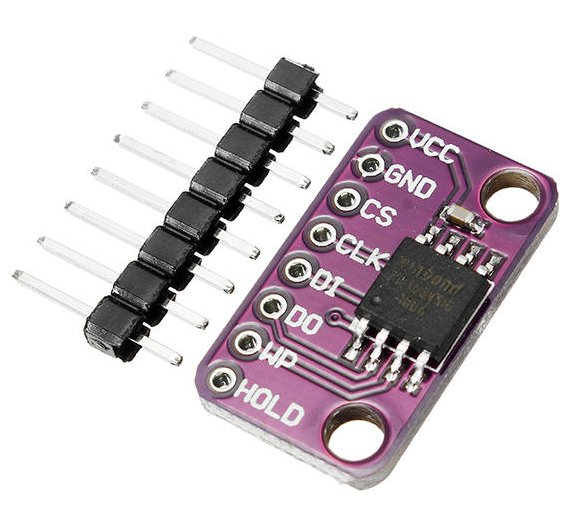
\includegraphics[scale=0.35]{./Figures/flash.jpg}
		\caption{Módulo flash basado en el circuito integrado W25Q16BVSIG\protect\footnotemark.}
		\label{fig:cuadradoAzul}
	\end{figure}

	\footnotetext{Imagen tomada de: \url{https://www.antratek.com/rfm95-lora-module}}
	
\end{itemize}

%----------------------------------------------------------------------------------------

\section{Planificación}

De acuerdo a los requerimientos planteados en al sección 2.1 y en función del diagrama en bloques general del dispositivo mostrado en la sección 2.2, se confeccionó una planificación de este trabajo como parte de la materia e Gestión de Proyectos de la carrera de Especialización.

\subsection{Actividades del trabajo}

El trabajo fue dividido en distintas actividades, cada una cumple con uno o varios de los requerimientos planteados previamente. En la figura 2.x se observa el diagrama AON (\textit{Activity On Node}, actividad en el nodo).

\begin{figure}[h]
	\centering
	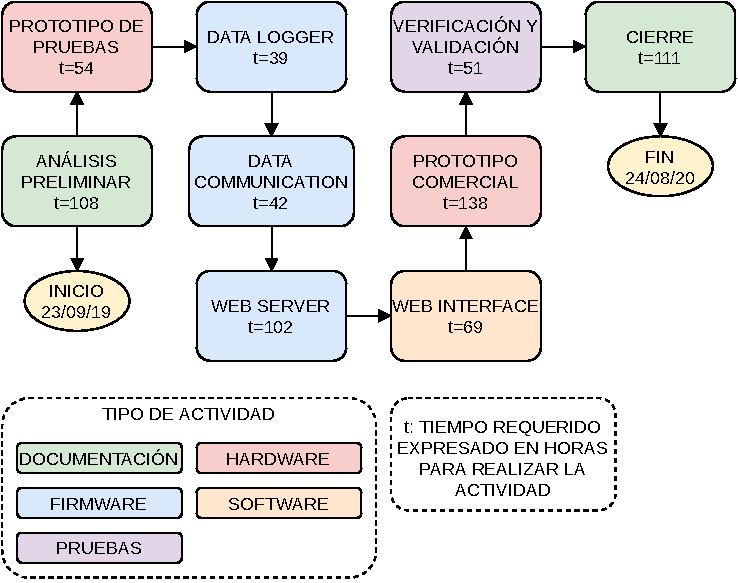
\includegraphics[scale=1]{./Figures/aon.pdf}
	\caption{Diagrama AON del trabajo.}
	\label{fig:diagramAON}
\end{figure}

Resalta que la cantidad de horas destinadas al desarrollo de firmware y hardware son aproximadamente el 62\% del tiempo previsto para el desarrollo trabajo en general. Esto guarda relación con el esfuerzo destinado para obtener resultados que garanticen un buen desempeño técnico del dispositivo desarrollado.

\subsection{Desgloce en tareas}

Para mejorar el control del tiempo que para el desarrollo de cada una de las actividades planteadas anteriormente, estas fueron desglosadas en tareas. Cada una de las tareas responden 

\subsection{Entregables del trabajo}

Los entregables del proyecto son los siguientes:
\begin{itemize}
	\item Diagrama esquemático.
	\item Código fuente.
	\item Prototipo comercial.
	\item Manual de instalación.
	\item Manual de uso.
	\item Informe final.
\end{itemize}

%----------------------------------------------------------------------------------------